%
% CSE Electronic Homework Template
% Last modified 8/23/2018 by Jeremy Buhler

\documentclass[11pt]{article}
\usepackage[left=0.7in,right=0.7in,top=1in,bottom=0.7in]{geometry}
\usepackage{fancyhdr} % for header
\usepackage{graphicx} % for figures
\usepackage{amsmath}  % for extended math markup
\usepackage{amssymb}
\usepackage[bookmarks=false]{hyperref} % for URL embedding
\usepackage[noend]{algpseudocode} % for pseudocode
\usepackage[plain]{algorithm} % float environment for algorithms

%%%%%%%%%%%%%%%%%%%%%%%%%%%%%%%%%%%%%%%%%%%%%%%%%%%%%%%%%%%%%%%%%%%%%%
% STUDENT: modify the following fields to reflect your
% name/ID, the current homework, and the current problem number

% Example: 
%\newcommand{\StudentName}{Jeremy Buhler}
%\newcommand{\StudentID{123456}

\newcommand{\StudentName}{Ming-Che Teng}
\newcommand{\StudentID}{466303}
\newcommand{\HomeworkNumber}{2}

%%%%%%%%%%%%%%%%%%%%%%%%%%%%%%%%%%%%%%%%%%%%%%%%%%%%%%%%%%%%%%%%%%%%%%%%
% You can pretty much leave the stuff up to the next line of %%'s alone.

% create header and footer for every page
\pagestyle{fancy}
\fancyhf{}
\lhead{\textbf{\StudentName}}
\chead{\textbf{\StudentID}}
\rhead{\textbf{Assignment \HomeworkNumber}}
\cfoot{\thepage}

% preferred pseudocode style
\algrenewcommand{\algorithmicprocedure}{}
\algrenewcommand{\algorithmicthen}{}

% ``do { ... } while (cond)''
\algdef{SE}[DOWHILE]{Do}{doWhile}{\algorithmicdo}[1]{\algorithmicwhile\ #1}%

% ``for (x in y ... z)''
\newcommand{\ForRange}[3]{\For{#1 \textbf{in} #2 \ \ldots \ #3}}

% these are common math formatting commands that aren't defined by default
\newcommand{\union}{\cup}
\newcommand{\isect}{\cap}
\newcommand{\ceil}[1]{\ensuremath \left\lceil #1 \right\rceil}
\newcommand{\floor}[1]{\ensuremath \left\lfloor #1 \right\rfloor}
\newcommand*{\Perm}[2]{{}^{#1}\!P_{#2}}%
\newcommand*{\Comb}[2]{{}^{#1}C_{#2}}%
\newcommand*{\Int}{\int\limits}
\usepackage{listings}
\usepackage{color}


\definecolor{dkgreen}{rgb}{0,0.6,0}
\definecolor{gray}{rgb}{0.5,0.5,0.5}
\definecolor{mauve}{rgb}{0.58,0,0.82}
\lstset{frame=tb,
  language=Java,
  aboveskip=3mm,
  belowskip=3mm,
  showstringspaces=false,
  columns=flexible,
  basicstyle={\small\ttfamily},
  numbers=none,
  numberstyle=\tiny\color{gray},
  keywordstyle=\color{blue},
  commentstyle=\color{dkgreen},
  stringstyle=\color{mauve},
  breaklines=true,
  breakatwhitespace=true,
  tabsize=3
}

%%%%%%%%%%%%%%%%%%%%%%%%%%%%%%%%%%%%%%%%%%%%%%%%%%%%%%%%%%%%%%%%%%%%%%

\begin{document}
\subsection * {Problems}

\begin{enumerate}

\item [\textbf{1.}]  

\textbf{Logistic and Find test error MATLAB implementation}

Part 1

In the Logistic function file, the for loop terminates either iteration reaches the max\_its or the gradient goes below the tolerance, in this setting is $10^{-3}$. And here's the report, 

\begin{table}[h!]
  \begin{center}
    \caption{$E_{in}$ and classification error with $10^{-3} tolerance$}
    \label{tab:table1}
    \begin{tabular}{l|c|c|r}
      \text{Maximum Iterations} & \text{10,000} & \text{100,000} & \text{1,000,000}\\
      \hline
      \text{Number of Iterations} &  \text{10,000} & \text{100,000} & \text{1,000,000}\\
      \hline
      \text{$E_{in}$} & \text{0.5847} & \text{0.4937} & \text{0.4352}\\
      \hline
      \text{$E_{class}\_train$} & \text{0.3092} & \text{0.2237} & \text{0.1513}\\
      \hline
      \text{$E_{class}\_test$} & \text{0.3172} & \text{0.2069} & \text{0.1310}\\
    \end{tabular}
  \end{center}
\end{table}

$E_{test}$ is generally lower than $E_{in}$ because $E_{in}$ is an estimation bounded by a loose upper bound, so the actual $E_{test}$ can be lower than the error estimation in training.
Moreover, if the gradient isn't below the tolerance, more iterations basically bring the result of lower error rate.

Part 2

The best result is when the maximum iteration is 1 million time, the $E_{test}$= 0.1310 and it takes 43.50 seconds to achieve the goal. By using \texttt{glmfit} function, the $E_{test}$ = 0.1103 and takes only 0.0015 seconds.

Part 3

Scaling the features by subtracting the the mean and dividing by the standard deviation for each of the features, $Z_{train} = \frac{X_{train} - \overline{X}_{train}}{\sigma_{train}}$ and $Z_{test} = \frac{X_{test} - \overline{X}_{test}}{\sigma_{test}}$
By setting a lower tolerance rate, means the number of iterations would decrease. Also, if the learning rate $\eta$ is larger, it means the function would take a huge step each time. Here's the table that, with a fixed $10^{-6}$ tolerance, changing the learning rate from $10^{-6}$ to $10^{-5}$, $10^{-4}$, $10^{-3}$, $10^{-2}$, $10^{-1}$.

\begin{table}[h!]
  \begin{center}
    \caption{$E_{in}$ and $E_{test}$ with $10^{-6} tolerance$ and different learning rate}
    \label{tab:table1}
    \begin{tabular}{l|c|c|c|c|c|c|c|r}
      \hline
      \text{$\eta$} & \text{$10^{-5}$} & \text{$10^{-4}$} & \text{$10^{-3}$} & \text{$10^{-2}$} & \text{$10^{-1}$}  & \text{$1$} & \text{$3$} & \text{$5$}\\
      \hline
      \text{Number of Iterations} &  \text{23,371,190} & \text{2,337,115} & \text{233,707} & \text{23,367} & \text{2,332} & \text{229}& \text{73}& \text{41}\\
      \hline
      \text{$E_{in}$} & \text{0.4074} & \text{0.4074} & \text{0.4074} & \text{0.4074} & \text{0.4074}& \text{0.4074}& \text{0.4074}& \text{0.4074}\\
      \hline
      \text{$E_{test}$} & \text{0.1034} & \text{0.1034} & \text{0.1034} & \text{0.1034} & \text{0.1034}& \text{0.1034}& \text{0.1034}& \text{0.1034}\\
      \hline
      \text{Execution\_Time (sec)} & \text{1091} & \text{102} & \text{10.23} & \text{1.0127} & \text{0.1016 }& \text{0.0104}& \text{0.0031}& \text{0.0017 }\\
    \end{tabular}
  \end{center}
\end{table}
 
I'm kind of surprise that, even if the learning rate is pretty large, compare to the previous experiment, with a lower tolerance rate, we can achieve a great $E_{in}$ and $E_{test}$. with fewer iterations and fewer execution time.




\end{enumerate}

\pagebreak

\subsection*{Problems}
\begin{enumerate}

\item[\textbf{2.}]

\textbf{LFD Problem 2.22}

First, rewrite the equation, 

\begin{equation}
\begin{aligned}
E_D[E_{out}(g^{(D)})] =& E_D[E_{x,y}[(g^{D}(x) - y(x))^2]]\\
=& E{x,y}[E_{D}[(g^{D}(x) - y(x))^2]]\\
=& E_{x,y}[E_{D}[(g^{D}(x)]^2 - 2 \overline{g}(x)y(x) + (y(x))^2]
\end{aligned}
\end{equation}

Then we continue to modify the equation, 

\begin{equation}
\begin{aligned}
E_{D}[(g^{D}(x)]^2 - 2 \overline{g}(x)y(x) + (y(x))^2
=& E_{D}[(g^{D}(x)]^2 - 2 \overline{g}(x)(f(x) + \epsilon) + (f(x) + \epsilon)^2\\
=& E_{D}[(g^{D}(x)]^2 - \overline{g}(x)^2 + (\overline{g}(x)^2 - 2\overline{g}(x) + f(x)^2) + \epsilon^2 - 2 (\overline{g}(x) + f(x))\epsilon\\
=& E_{D}[(g^{D}(x) - \overline{g}(x))^2] + (\overline{g}(x) - f(x))^2 + \epsilon^2 -2\epsilon(\overline{g}(x)-f(x))\\
=& var(x) + bias(x) + \epsilon^2 - 2\epsilon(\overline{g}(x)-f(x))
\end{aligned}
\end{equation}

Then we can put $E_{x,y}$ back to the equation,

\begin{equation}
\begin{aligned}
E_{D}[E{out}(g^{D})] =& E_{x,y}[var(x)] + E_{x,y}[bias(x)] + E_{x,y}[\epsilon^2] - 2E_{x,y}[(\epsilon(\overline{g}(x) - f(x)))]\\
=& var + bias + E_{x}[E_{y|x}[\epsilon^2|x]] - 2E_{x}[E_{y|x}[\epsilon(\overline{g}(x) - f(x)) | x]]\\
=& var + bias + E_{x}[E_{\epsilon}[\epsilon^2]] - 2E_{x}[\overline{g}(x) - f(x)E_{y|x}[\epsilon|x]]\\
=& var + bias + E_{\epsilon}[(\epsilon - E_{\epsilon}[\epsilon])^2] - 2E_{x}[(\overline{g}(x)-f(x))E_{\epsilon}[\epsilon]]\\
=& var + bias + \sigma^2
\end{aligned}
\end{equation}
 
\end{enumerate}

\pagebreak

\subsection*{Problems}
\begin{enumerate}
\item[\textbf{3.}]

\textbf{LFD Problem 2.24}

(a) 

\begin{equation}
\begin{aligned}
\overline{g}(x) =& E_{D}[g(x)]\\
=& E_{D}\Big[\frac{y_1-y_2}{x_1-x_2}x + \frac{x_1y_2-x_2y_1}{x_1-x_2}\Big]\\
=& \frac{1}{4} \int_{-1}^{1}\int_{-1}^{1}\frac{x_1^2 - x_2^2}{x_1-x_2}dx_1dx_2  \cdot x+ \frac{1}{4} \int_{-1}^{1}\int_{-1}^{1}\frac{x_1x_2^2 - x_2x_1^2}{x_1-x_2}dx_1dx_2\\
=& \frac{1}{4} \int_{-1}^{1}\int_{-1}^{1}(x_1 +  x_2)dx_1dx_2 \cdot x - \frac{1}{4} \int_{-1}^{1}\int_{-1}^{1}(x_1x_2)dx_1dx_2\\
=& 0
\end{aligned}
\end{equation}

(b)

We can simulate the process for, let's say 100 times, determining $\overline{g}(x)$, $E[E_{out}]$, $bias$, and $var$. The code on MATLAB is like 

\begin{lstlisting}
x = -1:0.00001:1;
y = x.^2;
z = 0 * x;
bias = 0;
Eout2 = 0.0;
var2 = 0.0;
for i = 1:10000
    var1 = 0;
    Eout1 = 0;
    rand1(i) = randperm(length(x),1);
    rand2(i) = randperm(length(x),1);
    randx1(i) = x(rand1(i));
    randx2(i) = x(rand2(i));
    randy1(i) = y(rand1(i));
    randy2(i) = y(rand2(i));
    m(i) = (randy1(i) - randy2(i))/(randx1(i) - randx2(i));
    b(i) = (randx1(i)*randy2(i) - randx2(i)*randy1(i))/(randx1(i) - randx2(i));
    for j = (1:length(x))
        if(x(j) ~= randx1(i))
            if(x(j) ~= randx2(i))
                var1 = var1 + (m(i)*x(j)+b(i) - 0)^2;
                Eout1 = Eout1 + (m(i)*x(j)+b(i) - y(j))^2;
            end
        end
    end
    var2 = (var1/199999) + var2;
    Eout2 = (Eout1/199999) + Eout2;
end
varAvg = var2/10000;
varRound = round(varAvg,2);
Eout = Eout2/10000;
EoutRound = round(Eout, 2);

for i = 1:200001
    bias = bias + (0 - y(i))^2;
end
biasAvg = bias/200001;
biasRound = round(biasAvg,2);
E_Eout = biasRound+varRound;

g_x = plot(x, m(1)*x + b(1), 'b--', 'LineWidth', 0.2)
hold on
for i = 2:10000
    plot(x, m(i)*x + b(i), 'b--', 'LineWidth', 0.2)
end
target_func = plot(x,y, 'r', 'LineWidth', 3)
gbar_func = plot(x,z, 'g', 'LineWidth', 3)
hold off
title('LFD Problem 2.24')
xlabel('x')
ylabel('y')
legend([target_func, gbar_func, g_x],'$y = x^2$','$\bar{g}(x)$','$g^{(D)}(x)$', 'Interpreter', 'latex', 'Location', 'SouthWest')
hold off
\end{lstlisting}

And the graph for the simulation is like,

\includegraphics[scale = 0.4]{/Users/alexteng/Desktop/CSE417/LFD2_24.pdf}


\pagebreak

(c)

Based on my simulation code, the length of $x$ and $y$ are 200001, and we sample 2 data points out of it for 10000 times. Each time we can formulate a linear hypothesis for predicting y. The result is showing below, 

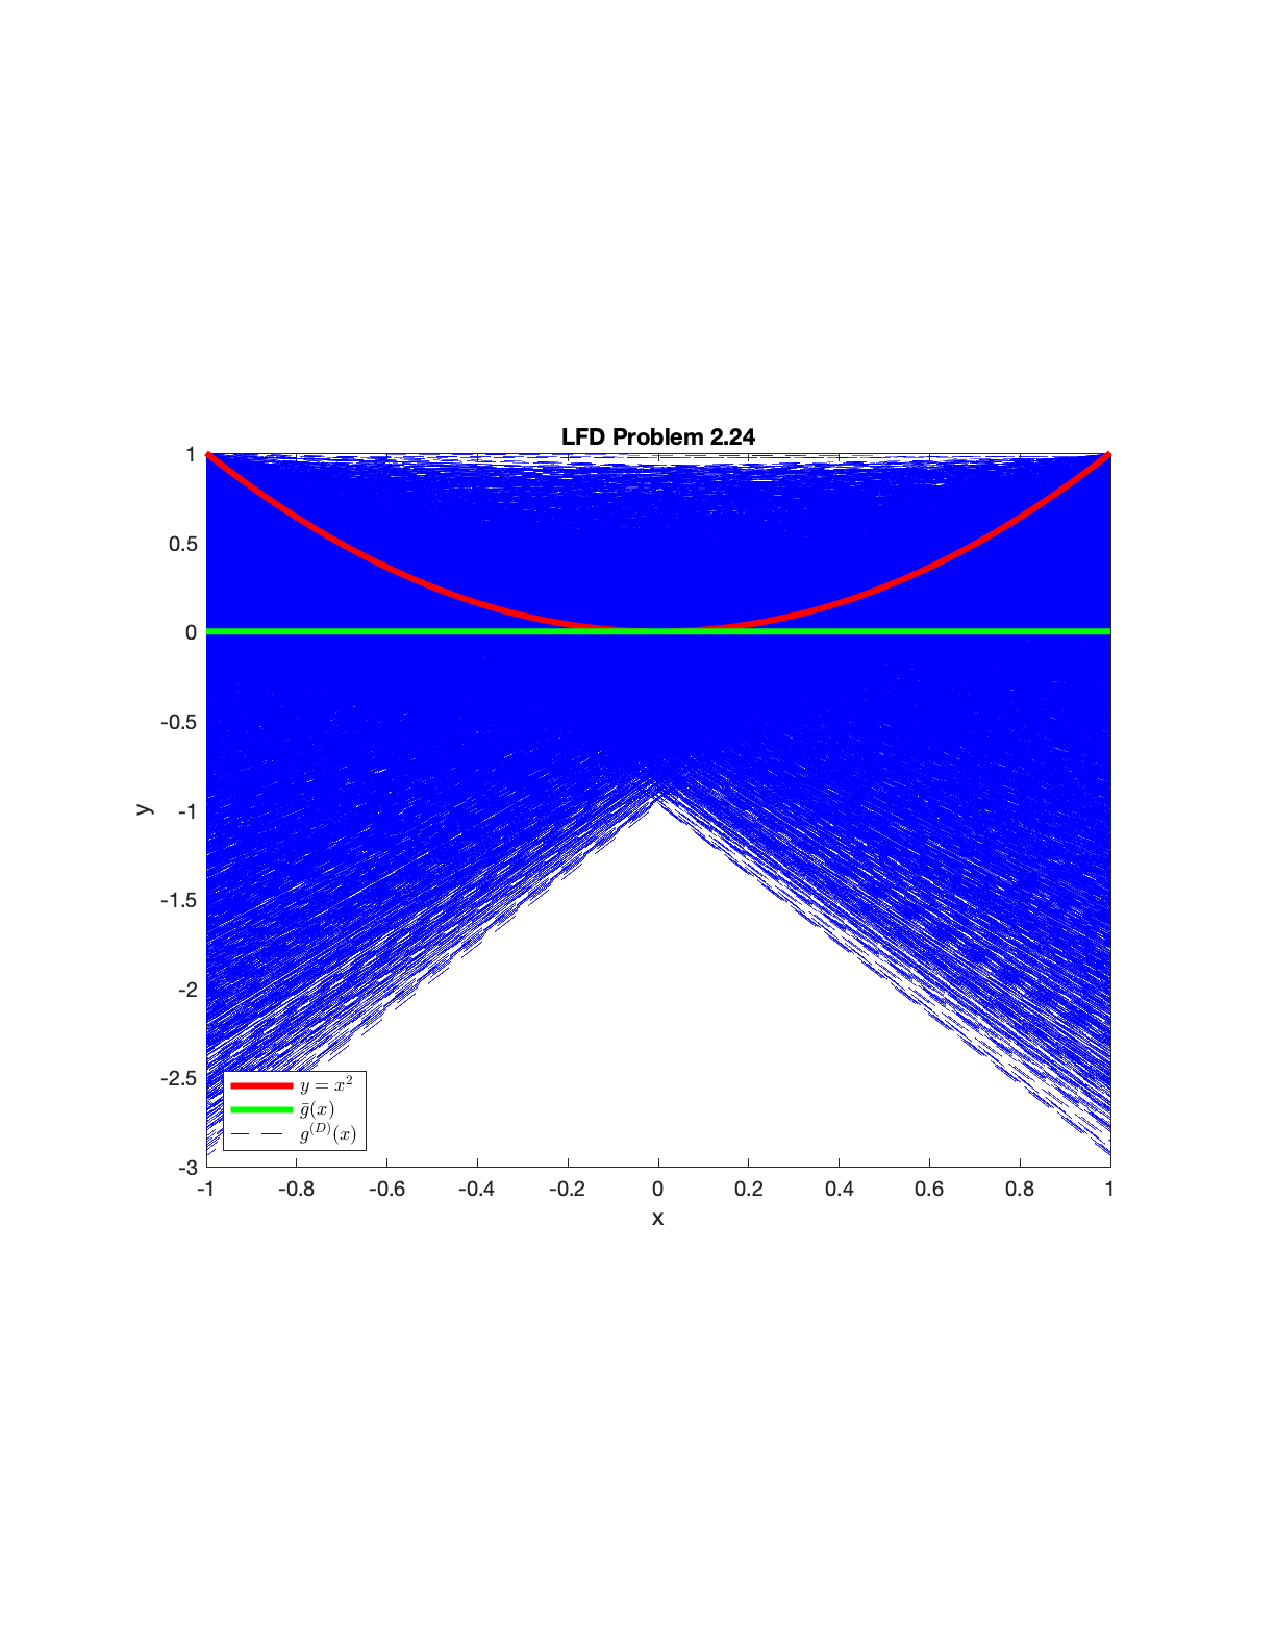
\includegraphics[scale=0.75]{/Users/alexteng/Desktop/CSE417/LFD2_24_C.pdf}

$E_{out}$ is the actual out-of-sample error, $E\_E_{out}$ means expected value of out-of-sample error which is calculated by sum of bias and variance. The result represents that $E_{out} = bias + var$

(d)

First, we compute $E_{out}$

\begin{equation}
\begin{aligned}
E_{out} = E[(g(x)-f(x))^2] =&E_x[(ax+b-x^2)^2]\\
=& E_x[x^4] -2aE_x[x^3]+(a^2 -2b)E_x[x^2]+2abE_x[x]+b^2\\
=& \frac{1}{2}\int_{-1}^{1}x^4dx-2a\frac{1}{2}\int_{-1}^{1}x^3dx+(a^2-2b)\frac{1}{2}\int_{-1}^{1}x^2dx+2ab\frac{1}{2}\int_{-1}^{1}xdx+b^2\\
=& \frac{1}{5} + \frac{(a^2-2b)}{3}+ b^2
\end{aligned}
\end{equation}

Then, we can take expectation with respect to $D$ to get the test performance, and replace $a$ and $b$ with $\frac{(y_1-y_2)}{(x_1-x_2)}$ and $\frac{x_1y_2 - x_2y_1}{x_1 - x_2}$ respectively, and, again, replace $y_1$ and $y_2$ with $x_1^2$ and $x_2^2$, we get,

\begin{equation}
\begin{aligned}
E_D[E_{out}] =& \frac{1}{5}+\frac{1}{3}E_D[(x_1+x_2)^2 + 2x_1x_2] + E_D[x_1^2x_2^2]\\
=&\frac{1}{5}+\frac{1}{3}\cdot \frac{1}{4}\int_{-1}^{1}\int_{-1}^{1}[x_1^2+x_2^2 + 4x_1x_2]dx_1dx_2 + \frac{1}{4}[x_1^2x_2^2]dx_1dx_2\\
=& \frac{1}{5}+\frac{1}{3}\cdot \frac{1}{4} \cdot \frac{8}{3} + \frac{1}{4}\cdot \frac{4}{9} = \frac{8}{15} \approx 0.53
\end{aligned}
\end{equation}

The we can compute the bias and variance, 
$$bias(x) = (\overline{g}(x)-f(x))^2 = x^4 = E[x^4] = \frac{1}{2}\int_{-1}^{1}x^4dx = \frac{1}{5}$$

\begin{equation}
\begin{aligned}
var(x) =& E_D[(g(x) - \overline{g}(x))^2] = E_D[a^2x^2 + 2abx + b^2]\\
=& E_D[a^2]x^2 + 2E_D[ab]x + E_D[b^2]\\
=& E_D[(x_1 + x_2)^2] x^2 - 2E_D[(x_1+x_2)x_1x_2]x + E_D[x_1^2x_2^2]\\
=& \frac{1}{4}\int_{-1}^{1}\int_{-1}^{1}(x_1^2 2x_1x_2 + x_2^2)dx_1dx_2 \cdot x^2 - \frac{1}{2}\int_{-1}^{1}\int_{-1}^{1}(x_1^2x_2+x_1x_2^2)dx_1dx_2\cdot x + \frac{1}{4}\int_{-1}^{1}\int_{-1}^{1}x_1^2x_2^2dx_1dx_2\\
=& \frac{1}{4}(\frac{4}{3}+0+\frac{4}{3}) \cdot x^2 - 0\cdot x + \frac{1}{4}\frac{4}{9} = \frac{2}{3}\cdot x^2 + \frac{1}{9}
\end{aligned}
\end{equation}

then take the expectation with respect to x,

$$var = E_x[\frac{2}{3}x^2 + \frac{1}{9}] = \frac{2}{3}\frac{1}{2}\int_{-1}^{1}x^2dx + \frac{1}{9} = \frac{1}{3}$$

$bias + var =  0.2 + \frac{1}{3} \approx 0.53$



\end{enumerate}

\pagebreak

\subsection*{Problems}
\begin{enumerate}

\item[\textbf{4.}]

\textbf{LFD Exercise 3.4}

(a)

Based on what we know, $y = Xw^{\ast}+ \epsilon$ from textbook,
\begin{equation}
\begin{aligned}
y =& Xw^{\ast}+ \epsilon\\
\hat{y} =& Hy\\
\hat{y} =& H(Xw^{\ast}+ \epsilon)\\
\hat{y} =& (X(X^TX)^{-1}X^T)Xw^{\ast}+ H\epsilon\\
\hat{y} =&  (XX^{-1}(X^T)^{-1}X^T)Xw^{\ast}+ H\epsilon\\
\hat{y} =& (II)Xw^{\ast}+ H\epsilon\\
\hat{y} =& Xw^{\ast}+ H\epsilon
\end{aligned}
\end{equation}

(b)

Simply replace $\hat{y}$ and $y$ with equation as below, 

\begin{equation}
\begin{aligned}
y =& Xw^{\ast}+ \epsilon\\
\hat{y} =& Xw^{\ast}+ H\epsilon\\
\hat{y} - y =& Xw^{\ast}+ H\epsilon - (Xw^{\ast}+ \epsilon)\\
=& (H-I)\epsilon
\end{aligned}
\end{equation}

where $I$ is an identity matrix.

(c)

Based on part(b) and the $E_{in}[W_[lin]] = \frac{1}{N}||\hat{y} - y||^2$, we can rewrite the equation, 

\begin{equation}
\begin{aligned}
E_{in}[W_{lin}] =& \frac{1}{N}||\hat{y} - y||^2\\
=& \frac{1}{N} ||(H-I)\epsilon||^2, \text{using the fact from part(b)}\\
=& \frac{1}{N} (\epsilon^TH^TH\epsilon - 2\epsilon^TH^T\epsilon +\epsilon^TI^TI\epsilon), \text{matrix algebra}\\
=& \frac{1}{N} (\epsilon^TH\epsilon - 2\epsilon^TH\epsilon + \epsilon^T\epsilon), \text{Using the fact that H are symmetric and $H^2 = H$}\\
=& \frac{1}{N} (-\epsilon^TH\epsilon + \epsilon^TI\epsilon)\\
=& \frac{1}{N} (\epsilon^T(I-H)\epsilon)\\
=& \frac{1}{N}\epsilon^T\epsilon - \frac{1}{N}\epsilon^TH\epsilon 
\end{aligned}
\end{equation}



\end{enumerate}
\pagebreak
\subsection*{Problems}
\begin{enumerate}

\item[\textbf{5.}]

\textbf{LFD Problem 3.4}

(a)

\[
e_{n}(w)
= \begin{cases}
0 & \text{if $y_nw^Tx_n > 1$}\\
(1 - y_nw^Tx_n)^2 & \text{if $y_nw^Tx_n < 1$}
\end{cases}
\]

and now we have, 

$$\lim_{w:y_nw^Tx_n \rightarrow \pm 1} e_n(w) = 0$$

which is the definition of continuous function.

Then we want to prove it's differentiable, 

\[
\triangledown e_n(w)
=\begin{cases}
0 & \text{if $y_nw^Tx_n > 1$}\\
-2y_n(1 - y_nw^Tx_n)x_n & \text{if $y_nw^Tx_n < 1$}
\end{cases}
\]

and we have, 

$$ \lim_{w:y_nw^Tx_n \rightarrow \pm 1} \triangledown e_n(w) = 0$$

shows that it's differentiable as well.


(b)

Now we list two functions we're interested in, 
\[
sign(w^Tx_n) \neq y_n 
= \begin{cases}
0 & \text{if $sign(w^Tx_n) = y_n$}\\
1 & \text{if $sign(w^Tx_n) \neq y_n$}
\end{cases}
\]

\[
e_{n}(w)
= \begin{cases}
0 & \text{if $y_nw^Tx_n > 1$}\\
(1 - y_nw^Tx_n)^2 & \text{if $y_nw^Tx_n < 1$}
\end{cases}
\]

Imagine if $sign(w^Tx) \neq y_n$, which means the equation $sign(w^Tx_n) \neq y_n) = 1$, and since the sign of $w^Tx_n$ is not equal to the sign of $y_n$, for the equation $e_{n}(w) = (max(0, 1-y_nw^Tx_n))^2$, the term $-y_nw^Tx_n$ now is positive. So the overall $1-y_nw^Tx_n$ is greater than 1. So the claim holds in this case.

Here's the mathematic expression,

\begin{equation}
\begin{aligned}
sign(w^Tx_n) \neq& y_n \rightarrow \text{$(sign(w^Tx_n) \neq y_n) = 1$}\\
-y_nw^Tx_n > 0& \rightarrow \text{$e_n(w) = (max(0,1- y_nw^Tx_n))^2 > 1$}
\end{aligned}
\end{equation}

The other case, when $sign(w^Tx_n) = y_n$, $(sign(w^Tx_n) \neq y_n) = 0$, and since the sign of $w^Tx_n$ is equal to $y_n$, for the equation $e_n(w) = (max(0,1-y_nw^Tx_n))^2$, the minimum value is 0, so the claim holds as well.

Here's the mathematic expression, 

\begin{equation}
\begin{aligned}
sign(w^Tx_n) = y_n \rightarrow \text{$(sign(w^Tx_n) \neq y_n) = 0$}\\
y_nw^Tx_n < 0 \rightarrow \text{$e_n(w) = (max(0,1-y_nw^Tx_n))^2 \geq 0$}
\end{aligned}
\end{equation}

Since for each n, $e_n(w) \geq (sign(w^Tx_n) \neq y_n)$, we can say $e_n$ is an upper bound for $sign(w^Tx_n) \neq y_n$, then we can have the function below, 

$$\frac{1}{N}\sum_{n=1}^{N}e_n(w)\geq \frac{1}{N}\sum_{n=1}^{N}(sign(w^Tx_n)\neq y_n) = E_{in}(w)$$

It's proved.

(c)

If we apply stochastic gradient descent on $\frac{1}{N}\sum_{n=1}^{N}E_n(w)$, we can get the following algorithm.

First, Select an initial $w$, 

Second, repeat until condition: select $(x_n, y_n)$ randomly and let $s_n = w^Tx_n$. If $y_ns_n \leq 1$, means $s_n$ is further from $y_n$ so we do the following

$$\triangledown e_n(w) = -2y_n(1-y_nw^Tx_n)x_n$$

and then update $w$ as

$$w(t+1) = w(t) + \eta \triangledown e_n(w) = w(t) + 2\eta y_n(1-y_ns_n)x_n = w(t) + \eta'(y_n - s_n)x_n$$

If $y_ns_n > 1$ means $s_n$ does well, and since $y_ns_n > 1$ will lead $e_n(w) = 0$, the $\triangledown e_n(w)$ is also 0, then, 

$$w(t+1) = w(t) + \eta \cdot 0 = w(t)$$, which means the algorithm does nothing. 

This whole algorithm is exactly Adaline algorithm.



 
\end{enumerate}
\pagebreak
\subsection*{Problems}
\begin{enumerate}
\item[\textbf{6.}]

\textbf{LFD Problem 3.19}

(a)

Let's say we have 3 data points, $x_1$, $x_2$, and $x_3$, based on the transformer, if all these three data points are different pairwise, then $x_1$ would be transformed to $(1,0,0)$.


We can imagine that, for this transformation, one potential problem is the complexity goes to infinity as n grows large. The other problem is, although it's not unusual to map each point not in the data set to 0, this is still a waste as n grows.

(b)

Using the example in part(a), we have 3 data points.

For this new transformer, and let's say we want to transform $x_2$, it becomes, 


\[
\Phi(x_2) = 
\begin{bmatrix}
e^{(-\frac{||x_2-x_1||^2}{2\gamma^2})}\\
e^{(-\frac{||x_2-x_2||^2}{2\gamma^2})}\\
e^{(-\frac{||x_2-x_3||^2}{2\gamma^2})}\\
\end{bmatrix}
=
\begin{bmatrix}
\phi_1(x_2)\\
\phi_2(x_2)\\
\phi_3(x_2)\\
\end{bmatrix}
\]

In this transformer, when our number of data points increase, the dimensionality also increases. So this may be a problem if we have infinite number of data, the space complexity for the transformer would be pretty complicated.

(c)

For this transformer, the potential problem is that if we only have 3 data points, then this transformer is quite a waste since it creates a matrix with size of ${101 \times 101}$. However, compared with the previous 2 transformers, this one is much better since we know the dimensionality is fixed, though might be a waste, and as the size of training data grows, we can still have decent space complexity that is not corresponded to the number of data we have.





\end{enumerate}
\end{document}